% Source: 2014江西文 PDF p.1 (printed893), Q10 option B.
% B is deliberately impossible for a common a. These two polynomials reproduce
% the option's qualitative geometry, not a solution of the parameter family.
% Cubic extrema x=-2.8,-.95; parabola vertex x=-.78 is to their right.
% For the stated family a<0, 1/a < 1/(2a) < 1/(3a), contradicting B.
\usetikzlibrary{arrows.meta}
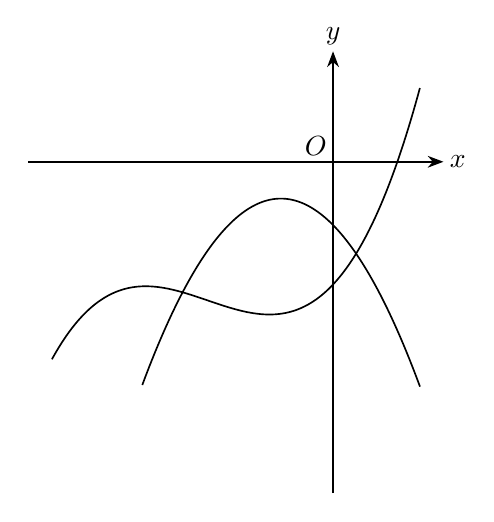
\begin{tikzpicture}[x=.85cm,y=.85cm,line width=.6pt,font=\normalsize,>=Stealth]
\draw[->] (-4.55,0)--(1.65,0) node[right,inner sep=0pt,xshift=2pt] {$x$};
\draw[->] (0,-4.95)--(0,1.65) node[above,inner sep=0pt,yshift=2pt] {$y$};
\draw[domain=-4.2:1.3,samples=161] plot (\x,{(2/15)*(\x)^3+.75*(\x)^2+1.064*\x-1.8338666667});
\draw[domain=-2.85:1.3,samples=121] plot (\x,{-.65*(\x+.78)^2-.55});
\node[anchor=south east,inner sep=0pt,xshift=-2pt,yshift=2pt] at (0,0) {$O$};
\end{tikzpicture}
